\subsection{Anforderungen des Auftraggebers}
Der Auftraggeber teilt seine Anforderungen in notwendige und optionale Ziele ein, welche nachfolgend aufgelistet werden. Als notwendige Ziele für das Projekt wurden folgende festgelegt.

\begin{itemize}
	\item Chatbot ist in Slack verwendbar
	\item Datenbank, welche Veranstaltungen und Zuweisungen der Mitglieder enthält
	\item Erfassung, welche Mitglieder wie viele Dienste gemacht haben
	\item Abfragefunktion ist für Termine vorhanden
	\item zeitgesteuerte, ereignisbasierte und manuelle Erinnerungsfunktion
	\item Einschränkung der Zielgruppe bzgl. Erinnerungen möglich
	\item einfache Bedienbarkeit
	\item Erweiterbarkeit des Projekts gegeben
	\item MIT-ähnliche Lizenzen für Drittanbietersoftware und -quelltext
	\item Dokumentation der Datenbank
	\item Unabhängigkeit der relevanten Daten vom verwendeten Bot
	\item Zukunftssicherheit
\end{itemize}


Die optionalen Ziele werden nachfolgend aufgeführt.
\begin{itemize}
	\item aus iCal Termine extrahieren
	\item Dienstplan aus Doodle-ähnlicher Umfrage erstellen
	\item Nutzerberechtigungen
	\item Steuerung über E-Mail
	\item containerbasierte Lösung
	\item Caching für schnellere Abfragen
	\item Backup-Strategie
\end{itemize}

% Hier schon das Usecase-Diagramm hin? - NEIN, hier kommt nur das rein, was Ferdi gesagt hat. Alles was wir selbst erarbeitet haben kommt danach.

\subsection{Festlegungen}
% Synonyme, Beschreibungen, Abgrenzungen für die Arbeit

Eine Menge an Terminen wird mit $T$ bezeichnet, Veranstaltungen mit $V$ und Sitzungen mit $S$.

\subsection{Anwendungsfalldiagramme}

??????????? Das klingt eher wie ein Vorwort für den Entwurf der Digaramme. ich würde hier nur Dinge rein schreiben, die sich über mehrere Kapitel erstrecken, so als "globale variablen"

Die auf den vorherigen Seiten zusammengetragenen obligatorischen Projektziele wurden zur besseren Überprüfung der Ziele in Anwendungsfälle umformuliert. Diese wurden entsprechend \autoref{usecase-auftrag} auf die Akteure \enquote{Bot} und \enquote{Auftraggeber} verteilt.
Der Auftraggeber ist hierbei Ferdinand Malcher als Vorsitzender des Studentenclubs \enquote{Stecker}, der \enquote{Bot} ist eine nicht näher spezifizierte Chatbot-Technologie, die aber bewusst als Akteur eingeführt wurde, da sie selbständig Aktionen ausführen soll.

????????????????ß Ich glaube nicht, dass Ferdi Vorsitzender ist, er und Robert sind Auftraggeber soweit ich weiß


\begin{figure}[htbp]
    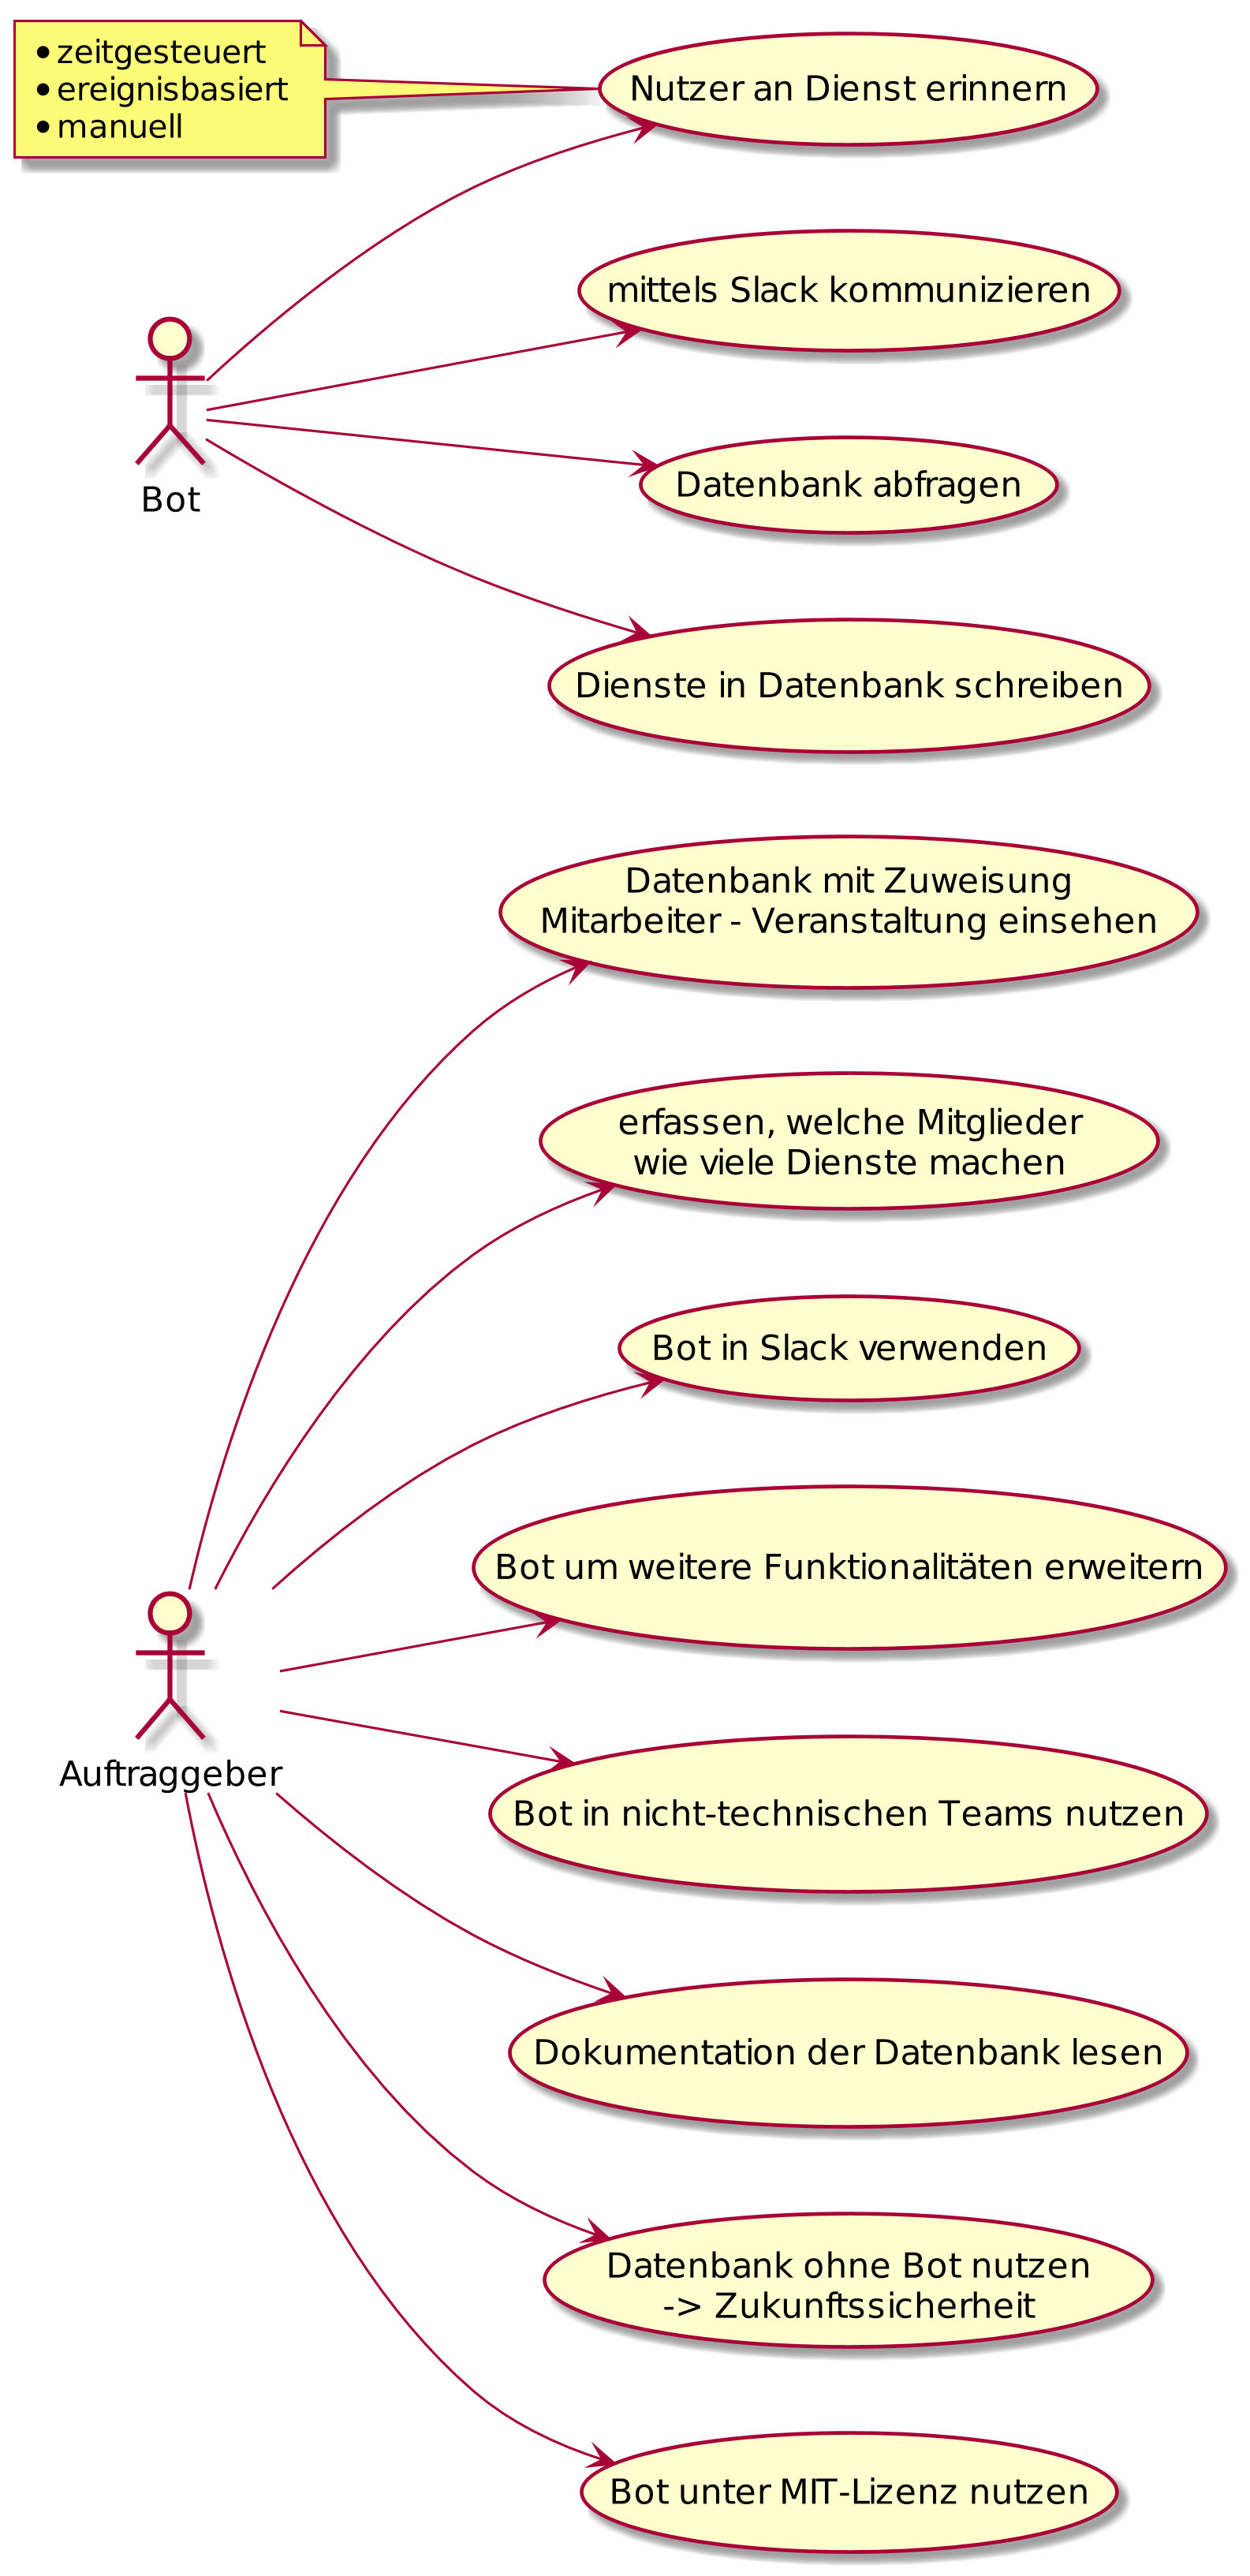
\includegraphics[width=0.7\textwidth]{../docs/uml/usecase-stakeholder.png}
    \caption{Anwendungsfalldiagramm für Auftraggeber und Bot}
    \label{usecase-auftrag}
\end{figure}

